\documentclass[11pt,a4paper]{article}
\usepackage[utf8]{inputenc}
\usepackage{amsmath}
\usepackage{amsfonts}
\usepackage{amssymb}
\usepackage{graphicx}
\usepackage{fancyhdr} %for header/footer
\author{platzh1rsch}
\title{Datennetze 1}
\author{Chregi Glatthard}
\date{3. Semester (HS 2012)}
\fancyfoot[C]{If you use this documentation for a exam, you should offer a beer to the authors!}

% hier beginnt das Dokument
\begin{document}

% Titelbild
\maketitle
\thispagestyle{fancy}

\newpage

\pagenumbering{Roman}
\tableofcontents	  	

\newpage

\setcounter{page}{1}
\pagenumbering{arabic}

\section{Datennetze}

\section{CCNA 1}
\subsection{Das Netz als eine Plattform}
Das Telefonnetz wurde für Sprachübermittlung (analog) konstruiert. In den 60er- und 0er-Jahren wurde es immer mehr digitalisiert. Parallel dazu enstanden in den 70er- und 80er-Jahren Computernetze. \linebreak
In den 90er-Jahren hat sich unter den Datennetzen das Internet für die breite Öffentlichkeit als Datennetz durchgesetzt.
\subsubsection{Was ist eigentlich "Internet"?}
Internet ist ein Netz das viele verschiedenartige lokale Netze miteinander verbindet. Es gibt standardisierte Kommunikationsregeln (TCP/IP).\linebreak
Datennetze werden in folgende 4 Elemente unterteilt:\linebreak
\begin{itemize}
\item Regeln
\item Nachrichten
\item Kommunikationskanal
\item Netzgeräte
\end{itemize}
\subsection{Dedizierte / Konvergierte Netze}
\subsubsection{Dedizierte Netze}
Früher baute man dedizierte (d.h. spezifische) Netze für eine Anwendung. Diese waren i.d.R. nicht miteinander kompatibel.
\subsubsection{Konvergierte Netze}
Mit der Zeit wurde es möglich verschiedene Dienste über ein Universalnetz zu transportieren. Diese Universalnetze nennt man konvergierte Netze.

\subsection{Architektur des Internets}
\subsubsection{Netzwerkarchitektur}
\begin{itemize}
\item Fehlertoleranz
\item Skalierbarkeit
\end{itemize}
\subsubsection{Vermittlung}
\begin{itemize}
\item Leitungsvermittlung
    \begin{itemize}
    \item konstant. und hohe Qualität
    \item schlechte Ausnutzung der Bandbreite
    \item limitierte Teilnehmerzahl
    \item Kosten
    \item limitierte Bandbreite
    \item Sicherheit
    \end{itemize}
\item Multiplexierung (TDM - Time Division Multiplex)
\item Paketvermittlung
    \begin{itemize}
    \item statistisch Multiplexen -> bessere Ausnutzung des Kanals
    \item günstiger
    \item mehr Overhead
    \item Verzögerung ist ein Problem -> kein QoS (Quality of Service)
    \item Sicherheit muss separat gewährleistet werden
    \end{itemize}
\end{itemize}

\section{Schichtenmodell}
Jedes Paket hat folgende Informationen:
\begin{itemize}
\item Absender
\item Ziel
\item zugehörige Anwendung
\item Nummer des Blocks
\end{itemize}
OSI - Open System Interconnection\linebreak
ISO - Standard Behörde (USA)\linebreak
MTU - Maximum Transmission Unit\linebreak
PDU - Protocol Data Unit (Header + Payload)\linebreak
\subsection{Protokolle}
Regelsammlung wie 2 Gegenüber kommunizieren sollen. Im Internet arbeiten verschiedene Protokolle zusammen und bilden so einen Protokoll-Stack

\subsection{Bekannte Anwendungsprotokolle}
\begin{tabular}{l c}
HTTP & 80 \\
FTP & 80, 81 \\
SSH & 22 \\
Telnet & 23 \\
DNS & 53 \\
\end{tabular}



\section{PacketTracer}
- Switches arbeiten mit MAC-Adressen nicht mit IPs
\section{Cisco}
Cisco Networking Academy: 
http://www.cisco.com/web/learning/netacad/index.html
CCNA


\section{CCNA 2}

\subsection{EIGRP}

\begin{figure}[h]
\begin{center}
	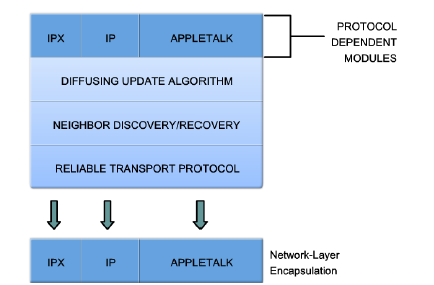
\includegraphics[scale=1]{img/EIGRP-Aufbau.png}
	\caption{Aufbau des EIGRP Protokolls}
	\label{a:label}
\end{center}	
\end{figure}

\begin{list}{-}{}
\item{klassenlos}
\item{Erweiterung IGRP (IGRP heute nicht mehr unterstützt)}
\item{CISCO proprietär}
\item{DV Protokoll}
\item{L3 Protokoll}
\end{list}


Unterschiede zu RIP 2:
\begin{list}{-}{}
\item{Diffusing Update Algorithm (DUAL) mit Link-State Protokoll Featuren}
\item{keine periodischen Updates}
\item{Nachbarschaftstabelle, Topologietabelle + Routingtabelle}
\item{sendet Hello-Pakete}
\item{altert Routen nicht mehr}
\item{Backup Routen}
\item{unterstützt neben IP auch andere L3 Protokolle als IP (z.b. IPX, 
AppleTalk usw.)}
\end{list}


Hauptziele:
- Robustheit (Routingschleifen vermeiden)
- Schnellere Konvergenz bei Änderungen im Netz
- Unterstützung auch anderer L3 Protokolle als IP

Zieldresse der Updates:
224.0.0.10
01-0-5E-00-00-0A

Nachrichtenformat:
- kein Transport-Header da L3 Protokoll

EIGRP Header
0		8		16				32
-----------------------------------------------------------------
| Version	| Opcode	|	Checksum		| 
-----------------------------------------------------------------
|			Flags					|
-----------------------------------------------------------------
|			Sequence				|
-----------------------------------------------------------------
|			Ack 					|
-----------------------------------------------------------------
|			Autonomous System			|
-----------------------------------------------------------------
|			Numbers					|
|			TLVs					|
-----------------------------------------------------------------

Opcode:	
Packet Type. 1 = Update, 3 = Query, 4 = Replay, 5 = Hello

Autonomous System Nr:
eher EIGRP Prozessnummer

EIGRP Payload:
TLVs (Type, Length, Values)

-------------
TLV 1 Parameter für die Metrik

TLV 2 Propagieren interner Routen
------------- > p 86 CCNA 2


----------------------------------

	Pakettypen

----------------------------------

Hello Pakete:
- Nachbarn finden und Nachbarschaften aufbauen
- werden unzuverlässig an Multicastadressen versendet

Update und Acknowledge Pakete:
- Updates nur gesendet wenn nötig
- nur notwendige Routinginformation
- zuverlässiger Transport
- Multicast für mehrere Empfänger, sonst Unicast

Query und Reply Pakete:
- Wenn DUAL Netze sucht, so werden Queries zuverlässig versendet
- Multicast / Unicast


Hello Protocol:
- bevor EIGRP Router Informationen austauschen kann, muss er 
Nachbarn erkennen und Nachbarschaften aufbauen
- Nachbarn müssen sich auf einem direkt angeschlossenen Netz 
befinden und EIGRP mit gleicher AS Nummer am Laufen haben
- Aufbau der Nachbarschaft mit Hello Paketen
- Hello Pakete alle 5s (Multicast Netze, z.b. Ethernet) bzw. alle 
60s (Point-to-Point Link)
- Holdtime besagt wie lange auf ein Hello eines Nachbarn gewartet 
werden soll bevor er für unerreichbar erklärt wird (standardmässig 
Holdtime = 3*Hello-Intervall)
- Wenn ein Nachbar für unerreichbar erklärt wird sucht DUAL einen 
neuen Pfad

Bounded Updates:
- EIGRP sendet "partial updates": Nur Infos über geänderte Routen 
werden gesendet
- "bounded updates": Updates nur an diejenigen Nachbarn welche von 
Änderung betroffen sind
--> Minimierung des Overhead Verkehrs

DUAL Algorithmus:
- sorgt dafür dass das Netz bei Änderungen möglichst schnell 
rekonfiguriert wird ohne Schleifen zu produzieren

---------------------------
Vorgang bei Änderung im Netz
---------------------------
- direkt an Router R angeschlossenes Netz wird unerreichbar
- R sendet Updates SOFORT an Nachbarn
- Nachbarn antworten mit ACK
- R sendet Anfrage ("Query") an Nachbarn ob anderer Weg zum Netz 
bekannt ist
- Nachbarn antworten mit ACK und prüfen ob anderer Weg zum betr. 
Netz bekannt ist, welcher ohne zu rechnen als neue Route 
eingetragen werden kann
	- ja? --> alternativer Weg eingetragen
	- nein? --> Netz wird auch bei Nachbar als unerreichbar 
markiert
- Nachbarn senden ihre Antwort ("Reply") und Router R sein ACK
- Falls kein Ersatzweg bekannt wird muss der verteilte 
Routingalgorithmus neu durchgerechnet werden

-------------------------------------------
Administrative Distanz und Authentisierung:
-------------------------------------------

AD von EIGRP:	90 für intern
		5 für Summary Routen
		17 für extern
		
Autonomous System:
Nummer des Netzes, wird normalerweise von ISP vergeben.
Alle Router im gleichen Netz müssen dieselbe AS Nummer haben, 
ansonsten können Sie nicht miteinander kommunizieren.


-------------------------------------------

	9.3 Berechnung der EIGRP Metrik

-------------------------------------------

EIGRP Metrik:
- Zusammengesetzt aus 4 Parametern:
	- Bandwith (statisch)
	- Delay (statisch)
	- Load
	- Reliability

Die Gewichtung der 4 Parameter wird mittels Konstanten festgelegt

metric weights tos k1 k2 k3 k4 k5	// Gewichtung der Metrik-
Parameter anpassen (aktuelle Konfiguration ersichtlich mit show 
ip protocols).

tos (Type of Service) ist Überbleibsel von IGRP, immer auf Null 
gesetzt.
Default-mässig werden nur die beiden statischen (k1 und k3) 
Parameter berücksichtigt.

----------------------
Metrik Parameter
----------------------

1. Bandwith
- Defaultwert: 1.54 Mbps (amerikanischer T1 Standard)
- kann sich von physik. Bandbreite unterscheiden
- durch clock rate festgelegt
- Bandbreite des langsamsten Links ist ausschlaggebend

2. Delay
- ähnlich wie Bandwith, kann sich vom tatsächlichen Wert 
unterscheiden
- Alle Delays aller Links zusammengezählt

z.b.	FastEthernet	100 micro-sec

3. Reliabilty
- Werte zwischen 0 und 255
- 25 entspricht keinen Bit-Fehlern, 0  = viele Bit-Fehler

4. Load
- Last
- 0 = wenig Verkehr
- 255 = Überlast

---------------------------------------------

	9.4 DUAL (Diffusing Update Algorithm)

---------------------------------------------

- Robustheit eines DV-Routingprotokolls hängt wesentlich von 
Konvergenzgeschwindigkeit ab
- deshalb nur Updates wenn Änderungen auftreten: Triggered Updates
- bei Leitungsunterbruch schnell Ersatzroute finden -> im Voraus 
berechnen und speichern

Successor:
- Router auf den die Route mit geringsten Kosten als nächster Hop 
zeigt ("next hop") in Routing-Tabelle nach "via"

Feasible Distance (FD):
- entspricht Kosten um an Ziel zu kommen
- wird in Routing-Tabelle als zweite Zahl in eckigen Klammern 
angezeigt
- entspricht "Metrik" in anderen Protokollen

Feasible Successor (FS):
- EIGRP Nachbar der sicher einen schleifenfreien Pfad zum Ziel hat 
und "feasibility condition" erfüllt

Reported Distance (RD) / Advertised Distance (AD):
- feasible distance eines Nachbarn zum Zielnetz


Feasibility Condition (FC)
- erfüllt wenn RD eines Nachbarn zu einem Ziel kleiner als FD des 
lokalen Routers
- verhindert Routing Schleifen

Für jede Parent Route wird in EIGRP eine Summary Route angelegt 
welche auf das IF Null0 führt. Dies führt dazu, dass Pakete welche 
zwar die Summary Route erfüllen aber keine ihrer Child Routen, 
verworfen wird.
Voraussetzungen:
- mind. ein Subnet wurde über EIGRP gelernt
- automatische Zusammenfassung ist nicht ausgeschaltet





\end{document}